%\linenumbers*
\chapter{ESTIMATION OF SOIL EROSION: IMPLICATIONS FOR FUTURE RAINFALL
INTENSITY}
\label{sec:ESTIMATIONSOFFUTURESOILEROSION}

\section{Introduction}
\label{sec:FutureSoilErosionIntroduction}

By acknowledging the limitation in investigating the effect of rainfall
intensity changes on future erosion rates, it is very unlikely that we will be
able to predict future rainfall intensity changes, and the effect on future soil
erosion with confidence.

If we knew with certainty what the impacts of climate change would be at a local
level, then adaptation would be easier; we could say this will be the impact in
this location in this year, and then look at what would need to happen to avoid
that impact. Unfortunately, we don't, and it is likely that we will never be
able to make predictions that are detailed enough and certain enough to make a
`predict and adapt' approach to adaptation a viable option.

However, it may still be possible to draw outlines of future erosion rates using
the findings from previous chapters. It may also be possible to simulate how
these future rainfall intensity changes will take place and affect soil
erosion.

This chapter aims to find out the impact of rainfall intensity changes on
``future'' soil erosion. The outcomes of this chapter aims to give answers for
Research Question \ref{researchquestion4}; \textit{Are we in a position to
predict erosion rates under future climates, with different rainfall intensities
from the present? If not, what must be done?}

%A simple answer to that question is no although how close they are capable
%of predicting would be another question.

As explained before, it is impractical to try to predict future erosion at this
stage because of the lack of reliable future rainfall data and the imperfection
of current erosion models that were found in the previous stages of this
research. It may be argued, however, that a guideline could still be drawn out
for investigating impacts of rainfall intensity changes on future erosion. In
this way, when rainfall data with an acceptable confidence level and better
intensity-aware erosion models become available, future erosion may be predicted
with a heightened certainty.

Only WEPP was utilised in this part of research because WEPP is the only
continuous simulation model from all three models used during this research. The
other two models (EUROSEM and RillGrow) are what is known as a single event
model that is only capable of dealing with a single rainfall event rather than
the whole system status that is dynamically updated as the simulation continues
over multiple rainfall events. A continuous simulation model---like WEPP---is
required to simulate long-term erosion without failing to consider the complex
overlap of temporally and spatially diverse distributions of rainfall,
erodibility, soil conditions, plant cover and so on \citep{nearing2006-145}.

Why did I do the last chapter even after I found that:
\begin{inparaenum}[1)]
 \item the requirement of data is great? We need very detailed rainfall data,
detailed enough to tell us about some intensity properties such as peak time and
gaps;
 \item observed data that are in high resolution has too much variability so
that drawing out trend is not feasible?
\end{inparaenum}

%\linenumbers*

%\chapter{FURTHER INVESTIGATIONS TO BUILD FUTURE RAINFALL INTENSITY SCENARIOS}
%\label{sec:FurtherInvestigationstoBuildFutureRainfallIntensityScenarios}

%\section{Proposed Simulation Methods}
\section{Possible Approaches to Simulating Future Rainfall Intensity}
\label{sec:ProposedSimulationMethods}

Despite the various efforts to find meaningful rainfall intensity trend for
building future scenarios of rainfall intensity changes, no significant trend
can be determined from analysing observed rainfall data in the study area.
Yet future rainfall intensities are predicted to increase.
%References and discuss why you did not find a trend (find it in CH3??)
However, even if the trend in rainfall intensity is available (for
example from an RCM), the results from this study indicate that knowing future
WSIV, WSIP and WSG is vital in order to carry out future erosion predictions. To
achieve the aim of this research, an alternative approach has to be sought to
obtain future rainfall data with a appropriate data resolution and
`changed' rainfall
intensity. The process of finding alternative approach is discussed in this
section.

%In order to predict changes of future rainfall intensity that are useful for
%estimating future soil erosion rates, it is vital to know how WSIV, WSG and
%WSIP are like in the future. However, even if we know these precisely for
%future, current models are not capable of utilising these properly because of
%the defects found previously (Section
%\ref{sec:EFFECTSOFCONTINOUSANDDISCONTINUSSTORM}).

%Thus, it has been suggested to analyse observed rainfall data to estimate a
%trend of rainfall intensity changes looking at a range of data scales. Based on
%the trend found, scenarios of future rainfall intensity were created.

%The analysis methods and the outcomes in this chapter are only presented to
%highlight limitations in our abilities to estimate future soil erosion rates.
%How future soil erosion may be estimated more adequately is also discussed in
%the latter section of this chapter.

%WEPP is used for the estimation of future soil erosion because only WEPP can
%perform continuous long term simulations.

\subsection{Approach 1: Changing CLIGEN Generated Data}
\label{sec:MethodOne}

%A similar method has been used in Section
%\ref{sec:MethodsSensitivityOfCLIGENToRainfallIntensityChanges}.
Daily peak rainfall intensity is changed by changing daily rainfall duration.
In a CLIGEN output, $R$, $D$, $t_p$ and $i_p$ comprise daily rainfall. These
are:
\begin{itemize*}
  \item $R$ : amount (inch)
  \item $D$ : duration (minute)
  \item $t_p$ : time to peak (normalised)
  \item $i_p$ : peak intensity (normalised)
\end{itemize*}
Among these four factors, duration ($D$) will be adjusted proportionally,
keeping other factors such as $t_p$, $i_p$ and $R$ constant. In this way, the
rainfall amount is kept constant, and rainfall intensity is varied.

Thirty year-long climate data were generated using CLIGEN with an input file,
which was prepared from the Southover dataset. Daily rainfall durations in this
30 year-long climate data were adjusted proportionally to obtain increased or
decreased daily peak rainfall intensities. Using the original and adjusted
climate data, runoff and soil erosion were to be simulated for 30 years. The
effect of \textit{indirect} rainfall intensity changes on runoff and erosion
were then analysed.

\paragraph{Pros:}
\label{sec:ProsMethodOne}
Simple, easy and fast.
%need more better justification
\paragraph{Cons:}
\label{sec:ConsMethodOne}
It may be considered to be crude and simple for simulating future rainfall
intensity changes. One reason is that it is not possible to change the number
of raindays using this approach. It does not make a full use of the findings
from the previous analyses. This is an indirect approach.

\subsection{Approach 2: Changing {MX.5P}, One of CLIGEN Input
Parameters}
\label{sec:MethodTwo}

\paragraph{Description of {MX.5P} (Yu, personal communication 2003)}
\label{sec:MX5PByBYu}

{MX.5P} is defined as ``Average maximum 30-min peak intensity (in/hr) for each
month''. If the sub-daily interval is denoted as $\Delta t$ (min), then there
are 1440/$\Delta t$ intervals, called $M_t$, in a day. For each wet day, discard
all the dry intervals to create a single storm event with \emph{continuous} rain
for, say, $M$ intervals. Then the storm duration, $D$, (min) is given by:
\begin{eqnarray}
  D = M \Delta t \delta
\end{eqnarray}

Find the maximum precipitation intensity for any 30-min period within the storm,
and call this $I_{30}$. If there are $n$ wet days in a month, find the maximum
of these $n$ $I_{30}$ values, and denote this maximum $I_{30}$ for the month as
$maxI_{30}$. If there are $K$ months on record, then {MX.5P} is given by:
\begin{eqnarray}
  \mathrm{MX.5P} = \frac{1}{K} \sum maxI_{30}
\end{eqnarray}

For example, let us say it rained on 3rd and 10th of May, 2001 with a peak
30-min intensity of 1.2 in/hr and 1.5 in/hr, respectively. Then $maxI_{30}$
would be 1.5 in/hr for May 2001. If we have 5 years of data for May:

\begin{table}[hbpt]
  \centering
  \begin{tabular}{ccc}
    \toprule
    Month & Year & $maxI_{30}$ (in/hr)\\
    \midrule
    May & 1997 & 0.8\\
    May & 1998 & 0.9\\
    May & 1999 & 0.3\\
    May & 2000 & 2.8\\
    May & 2001 & 1.5\\
    \bottomrule
  \end{tabular}
\end{table}

Then the {MX.5P} value for May for this hypothetical site would be:
\begin{equation}
  \frac{0.8+0.9+0.3+2.8+1.5}{5} = 1.26 \ \textrm{(in/hr)}.
\end{equation}

\paragraph{Changing {MX.5P}} The CLIGEN \emph{input} file was adjusted
accordingly rather than the CLIGEN
\textit{output} file. Two CLIGEN input files were prepared as if they are from
two different periods---present and future---of the site. Future climate changes
are thus conceptualised here as ``two different climate conditions in the same
place''. The original input file was built using observed event rainfall data
from Ditchling Road station. Rainfall intensity parameter ({MX.5P}) of the
original input file was adjusted accordingly to represent future rainfall
intensity changes (Table \ref{tab:MX5PChanges}). Two sets of CLIGEN-generated
weather data using these two input files only differ in peak rainfall
intensities, which is controlled by {MX.5P}. Then, WEPP simulates runoff and
soil
loss rates using these two CLIGEN climate data.

\begin{table}[htpb]
  \figureversion{tabular}
  \centering
  \caption{Ratio of {MX.5P} changes for each month}
  \label{tab:MX5PChanges}
    \begin{tabular}{lcccc}
    \toprule
    & \multicolumn{2}{c}{Decrease} & \multicolumn{2}{c}{Increase} \\
    \cmidrule(r){2-3} \cmidrule(l){4-5}
    Wet Season (SONDJF months)   & $-$10\% &  $-$5\%  & $+$5\%  & $+$10\% \\
    Dry Season (MAMJJA months)   & $-$10\%  & $-$5\%  & $+$5\%  & $+$10\% \\
    \bottomrule
    \end{tabular}
\end{table}

Few studies pointed out that the ratio of wet and dry days will influence the
behaviour of future soil erosion
\citep{nearing2001-229,pruski2002-climate,pruski2002-7}. However, as this thesis
only concentrates on the implication of rainfall intensity changes, no rainfall
frequency change is considered. No rainfall amount change is also assumed here.
Due to the lack of information, no intra-storm rainfall intensity pattern for
the future was considered.

Nearing (personal e-mail communications, 8 June 2001) pointed out that, if
MEAN~P in CLIGEN input file is changed together with {MX.5P}, we would end up
with completely different climate data from what we have started with. Also,
generated data may not have clear relationships with original data. This is a
problem for a sensitivity-type comparison---that is, comparing how WEPP
estimates differ for two well-defined sets of input data. On the other hand,
when creating ``realistic'' future rainfall data is to be the main concern, both
parameters (MEAN~P and {MX.5P}), together with other parameters may need to be
changed. It will, however, only be applicable to the case where sufficient
reference data are available for the adjustment and comparison of all the
parameter. No such information has been available for this research. Therefore,
until such information is available, it is important to limit the changes only
to a single parameter, {MX.5P} in this case, and carry out only the
sensitivity-type comparison.

It is very unlikely all the months will have the same changes in rainfall
intensity. There will be some degrees of variations depending on seasons, for
example. Two seasonal variations are considered here---Wet and Dry season. The
wet season includes September, October, November, December, January and February
(Table \ref{tab:AdjustedMX5Pvaluesforwetseasons}). The dry season consists of
March, April, May, June, July and August (Table
\ref{tab:AdjustedMX5Pvaluesfordryseasons}).

\begin{table}[htbp]
  \figureversion{tabular}
  \centering
  \footnotesize
  \caption{Adjusted {MX.5P} values for the wet season}
  \label{tab:AdjustedMX5Pvaluesforwetseasons}
    \begin{tabular}{r|cc|cccccc|cccc}
      \toprule
      month & \textbf{1} & \textbf{2} & 3 & 4 &5& 6& 7& 8& \textbf{9}
&\textbf{10}& \textbf{11}& \textbf{12}\\
      \midrule
      $-$10\% & 0.24 & 0.16 & 0.23 & 0.23&  0.27 & 0.33 & 0.42 & 0.58 & 0.39 &
0.41 & 0.31 & 0.27\\
      $-$5\%  &0.26 & 0.17 & 0.23 & 0.23 & 0.27 & 0.33 & 0.42 & 0.58 & 0.41 &
0.43 & 0.32 & 0.28\\
      original & 0.27 & 0.18 & 0.23  &0.23 & 0.27 & 0.33 &0.42 & 0.58 & 0.43 &
0.45 & 0.34 & 0.30\\
      5\% & 0.28 & 0.19 & 0.23 & 0.23 & 0.27 & 0.33 & 0.42& 0.58 & 0.45 & 0.47 &
0.36 & 0.32\\
      10\% & 0.30 & 0.20 & 0.23 & 0.23 & 0.27 & 0.33 & 0.42 & 0.58 & 0.47& 0.50
& 0.37 & 0.33\\
      \bottomrule
    \end{tabular}
\end{table}

\begin{table}[htbp]
  \figureversion{tabular}
  \centering
  \footnotesize
  \caption{Adjusted {MX.5P} values for the dry season}
  \label{tab:AdjustedMX5Pvaluesfordryseasons}
    \begin{tabular}{r|cc|cccccc|cccc}
      \toprule
      month & 1 &2& \textbf{3} &\textbf{4} &\textbf{5}& \textbf{6}& \textbf{7}&
\textbf{8}& 9 &10& 11& 12\\
      \midrule
      $-$10\%  &0.27&  0.18  &0.21 & 0.21 & 0.24 & 0.30 & 0.38 & 0.52 & 0.43 &
0.45 & 0.34&  0.30\\
      $-$5\% & 0.27 & 0.18 & 0.22  &0.22  &0.26  &0.31 & 0.40& 0.55 & 0.43 &
0.45 & 0.34 & 0.30\\
      original&  0.27  &0.18 & 0.23  &0.23 & 0.27 & 0.33 &0.42  &0.58 & 0.43&
0.45 & 0.34 & 0.30\\
      5\%  &0.27 & 0.18&  0.24& 0.24 & 0.28 & 0.35 & 0.44 &0.61 & 0.43 & 0.45 &
0.34 & 0.30\\
      10\% & 0.27  &0.18 & 0.25  &0.25  &0.30  &0.36 & 0.46& 0.64 & 0.43 &0.45
&0.34  &0.30 \\
      \bottomrule
    \end{tabular}
\end{table}

Since soil erosion is closely related to the extreme rainfall events, this
thesis concentrates on extreme rainfall events which are closely related to the
rainfall parameter, {MX.5P}. This is the main reason why {MX.5P} is chosen to be
altered. It is clear that \citet{nicks1995-2} has recognised the close
statistical relationship between {MX.5P} and soil erosion rate. Thus, it is
unsurprising that this parameter is explicitly included in the CLIGEN input
file.

\paragraph{Pros:}
\label{sec:ProsMethodTwo}
The procedures are relatively easy and uncomplicated. Calculating {MX.5P} is
relatively straightforward from tipping-bucket data. It does change the rainfall
intensity of extreme events.

\paragraph{Cons:}
\label{sec:ConsMethodTwo}
Generated rainfall data for the original and ``future'' climate are almost the
same except for rainfall intensity. Thus the ``future condition'' here is not,
physically, very realistic. Future climate will change in complex ways, not
only extreme rainfall intensity will change, but also probabilities of raindays,
WSIP (Within-Storm Intensity Pattern) and rainfall amount will very
probably also change.
Also, even if we increase or decrease extreme rainfall intensity only, the
intensity of small rainfall events are also affected in order to keep overall
annual rainfall amount constant.

\subsection{Approach 3: Using GCM/RCM Data}
\label{sec:MethodThree}

This third approach described here was proposed originally, but has not been
used
because there were no GCM data which were suitable for this research because of
the scale mismatch.
% (see Chapter \ref{sec:LimitationsOfErosionModels}) -- is this relevant?.
Nevertheless, daily RCM data for current and future climate have been acquired.
RCM also produced 20-min rainfall data, but with a high variability. Daily
rainfall intensity (or amount) is not suitable to be used as erosion model input
directly unless downscaled.

The procedures of this approach are:
\begin{enumerate*}
  \item GCM data with 30-min time step for current and future climate
  \item CLIGEN input files for current and future climate are built
  \item CLIGEN generates climate data for current and future climate
  \item WEPP simulates runoff and erosion for current and future climate.
\end{enumerate*}

It might be possible to calculate all the CLIGEN input parameters out of the GCM
output. GCMs can generate current and future climate data on a
sufficient temporal
resolution---that is, 30-min time step---for building CLIGEN input files.
This will permit a ``better''---in the sense of being more realistic---judgement
of impacts of rainfall intensity changes on future soil erosion.

%There are some possible caveats with this approach.
%One is that these high-resolution model-generated GCM data may have
%problems and errors caused by unconventional configurations on the top of GCMs'
%uncertainty and wide range of variations.
A major caveat is that the high resolution GCM data are still not readily
available. A separate model configuration is required to generate this
kind of data, and the set-up process usually requires extended model set-up
skills and simulation times. This was the case for the current research.
Another possible problem is that, because of the preceding uncertainty of GCM
output, we might end up with erroneous CLIGEN input files which, in turn, will
lead to even greater errors for future erosion estimation.

%summary table here

\subsection{Conclusion: Selected Approach}
\label{sec:SelectedMethod}

Approach 2 (Section \ref{sec:MethodTwo}) is selected. The schematic
procedure of this approach is shown in Figure
\ref{fig:future_erosion_flowchart}.
It was assumed that future WSIV, WSG and WSIP are the same as the present. Only
monthly maximum of 30-min peak rainfall intensity was considered for
constructing future rainfall intensity scenarios.

CLIGEN generates original climate data using the input file which statistically
represents the characteristics of current rainfall intensity. Keeping all other
parameters constant, the intensity parameter ({MX.5P}) in the CLIGEN input file
are increased or decreased proportionally (Table \ref{tab:MX5PChanges}).
{MX.5P} is specifically related to extreme intensity events as given by its
definition, `Average maximum 30 minutes peak intensity (in/hr) for each month'.
``Future'' climate data are then generated using adjusted CLIGEN input file.
WEPP simulates runoff and soil loss using both climate data. Runoff and soil
loss changes are compared with changes in rainfall intensity.

\begin{figure}[htpb]
  \centering
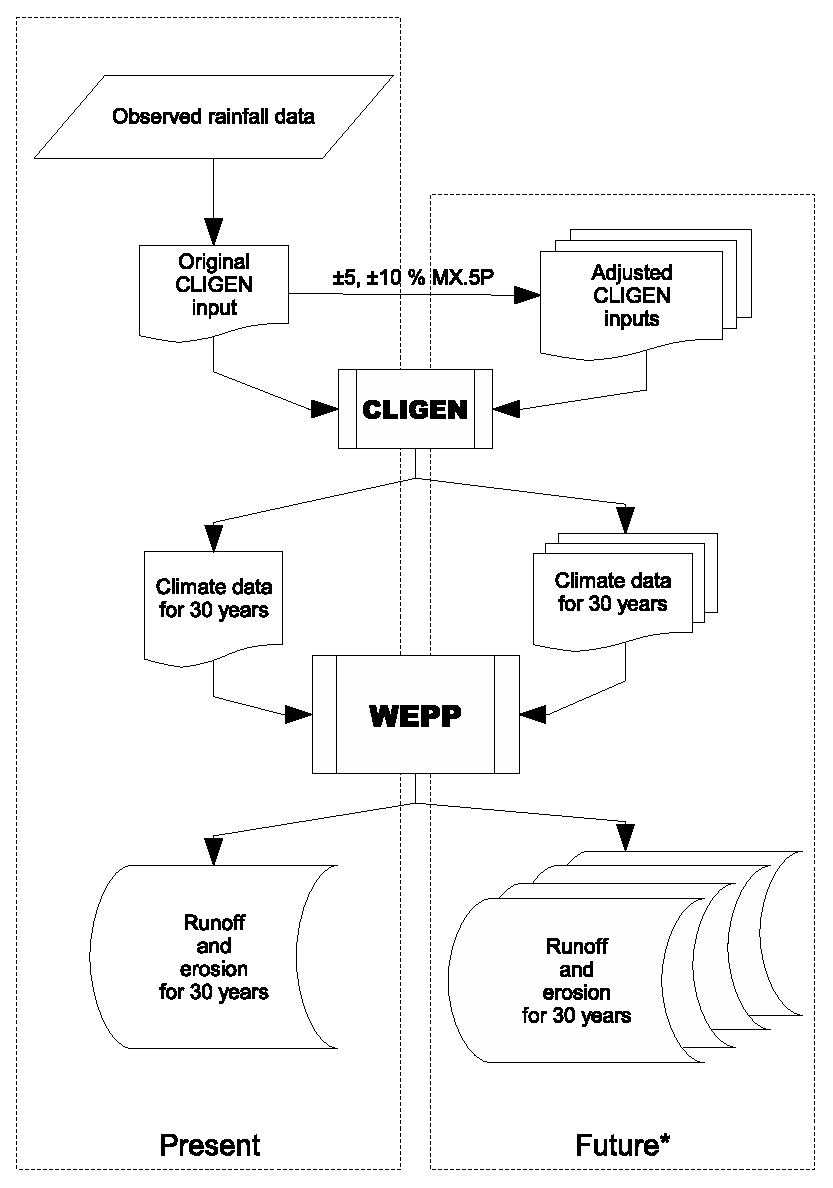
\includegraphics[width=0.8\textwidth]{./img/future_erosion_flowchart}
  \caption[Schematic flowchart of the approach used for investigation of
implications of rainfall intensity changes for future soil erosion]{Schematic
flowchart of the approach which is used for investigation of implications of
rainfall intensity changes for future soil erosion. Soil erosion simulated in
the left-side box marked with `Present' represents the present erosion rate
under current rainfall intensity. Soil erosion simulated in the right-side box
marked with `Future*' represents assumed future erosion rates under the
different rainfall intensities.}
  \label{fig:future_erosion_flowchart}
\end{figure}

%\nolinenumbers


\section{Sensitivity of WEPP to Rainfall Intensity Changes}
\label{sec:MethodsSensitivityOfCLIGENToRainfallIntensityChanges}

Before using WEPP for the current investigation, the sensitivity of WEPP to
changes in rainfall intensity were tested. Rainfall intensity was modified
indirectly by controlling the rainfall duration. The rainfall amount and ratio
of average intensity to peak intensity were not changed. The relationship
between actual peak intensity, $I$ and rainfall duration, $D$ can be described
as:
\begin{equation}
\label{eq:ActualIntensity}
  I = i_p \times \frac{R}{D}
\end{equation}
where $i_p$ is normalised peak intensity, $R$ is rainfall amount.

The rainfall amount, $R$, and normalised peak intensity, $i_p$, are parametrised
in a CLIGEN input file as station specific parameters (i.e. MEAN~P and MX~.5P),
so that they should not be changed directly from a CLIGEN output file. On the
other hand, rainfall duration, $D$, is generated by CLIGEN in relation to $R$
and $i_p$ values. Thus, \textit{only} daily peak rainfall intensities are
increased or decreased by decreasing or increasing rainfall duration while
keeping the rainfall amount constant (Table
\ref{tab:PeakRainfallIntensityChangesForWEPPSimulation}). All other factors,
such as rainfall frequency and seasonal intensity variation, are unchanged.

\begin{table}[htbp]
  \figureversion{tabular}
  \centering
  \caption[Peak rainfall intensity changes for WEPP simulation]{Peak
rainfall intensity changes (\%) for WEPP simulation}
  \label{tab:PeakRainfallIntensityChangesForWEPPSimulation}
    \begin{tabular}{lccccccc}
    \toprule
    Duration & 142.9 & 125.0 & 111.1 & 100 & 90.9 & 83.3 & 76.9\\
    \midrule
    Peak Intensity & 70 & 80 & 90 & 100 & 110 & 120 & 130\\
    \bottomrule
    \end{tabular}
\end{table}

Runoff and soil loss amount were estimated by WEPP (v2004.7). CLIGEN (v5.2) was
used to generate weather data using updated Ditchling Road input (see Appendix
\ref{sec:UpdatedInputForDitchlingRoad}). Calibrated WEPP was used as previously
reported. The resulting annual runoff and soil loss rate were analysed to find
out whether WEPP is sensitive to rainfall intensity changes.

\subsection{Runoff and Soil Loss}
\label{sec:SensitivityOfWEPPToRainfallIntensityChangesResults}
The mean annual soil loss estimated by WEPP increases or decreases as peak
intensity increases or decreases (Figure
\ref{fig:wepp_respond_to_int_changes}). WEPP is sensitive to daily peak
intensity changes with the rate of $\beta = 1.46$ ($y = \alpha + \beta x$).
This means that for each 1\% increase or decrease in daily peak intensity,
WEPP estimates a 1.46\% increase or decrease in the annual soil loss. The
annual runoff rate is slightly less sensitive to the changes in peak
rainfall intensity than annual soil loss
\ref{fig:wepp_respond_to_int_changes}.

\begin{figure}[htbp]
  \centering
    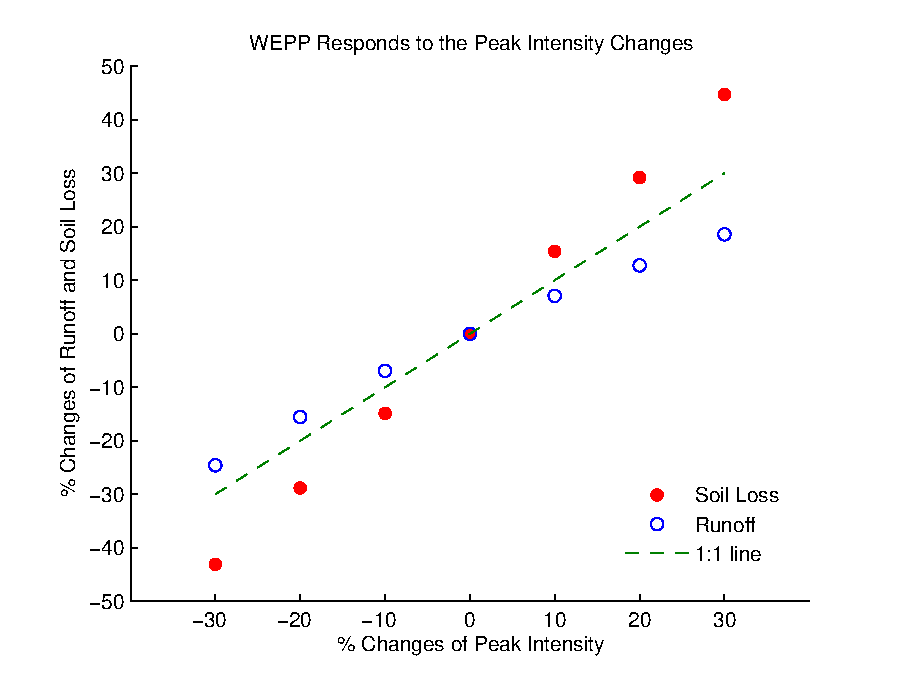
\includegraphics[width=0.70\textwidth]
{./img/wepp_respond_to_int_changes}
  \caption{WEPP responses to the peak rainfall intensity changes}
  \label{fig:wepp_respond_to_int_changes}
\end{figure}

\subsection{Discussion}
\label{sec:SensitivityOfWEPPToRainfallIntensityChangesDiscussion}
As the result implies, WEPP is sensitive to a change in rainfall intensity.

Although the method used here is arguably simple and crude, it serves the aim of
this study. It clearly shows the sensitivity of WEPP to rainfall intensity
changes. However, the resultant change in rates of soil loss in response to the
daily peak rainfall intensity is rather difficult to accept.

This is due to the following reasons:
\begin{itemize}
  \item This is an indirect approach to changing rainfall intensity.
  \item The normalised daily peak intensity parameter, $i_p$, has not been
changed. Thus, the relative magnitude of daily peak intensity to the daily
average intensity is the same.
  \item No seasonal variation is considered as every rainfall duration is
perturbed with the same change rate.
\end{itemize}

Moreover, when the same changes were applied to daily rainfall durations across
the data period, some of the events became extended over 24 hour period. These
events however were forced to be 24 hour events. This, however, did not affect
the final results.

WEPP may be used for the investigation, \textit{Estimation of Future Soil
Erosion}. However, it is important to keep in mind the limitations discussed
previously (see Section \ref{sec:LimitationsOfErosionModels}).

%No conclusion may need as there will be one ``conclusion'' for the whole
%chapter.

\section{Estimation of Future Soil Erosion}
\label{sec:MethodsEstimatedFutureSoilErosion}

As pointed out previously, our ability to predict future soil erosion is largely
limited by the shortcomings of GCMs. At the time of writing, magnitudes of
future rainfall intensity changes are not yet clearly quantified. Nevertheless,
it is evident that the observed frequency of heavy rainfall has increased in the
region of 2--4\% over the latter half of the 20th century \citep{ipcc2001-881}.

However, this still does not provide sufficient detail in rainfall information
required by the soil erosion models used here. In this research, it has been
shown that temporal scales of rainfall data, intra-storm intensity pattern and
continuity of rainfall duration affect soil erosion, and it is necessary to know
these information in order to estimate soil erosion adequately. The effect of
these factors on soil erosion are discussed previously (Chapter
\ref{sec:EFFECTSOFTEMPORALSCALESOFSTROMDATA}, Chapter
\ref{sec:EFFECTSOFRAINFALLINTENSITYCHANGESONSOILEROSION} and Chapter
\ref{sec:EFFECTSOFCONTINOUSANDDISCONTINUSSTORM}).

In order to investigate the impacts of future rainfall intensity changes on soil
erosion, it is undoubtedly necessary to know what future rainfall intensity is
like, and then apply these rainfall intensity changes to soil erosion models to
estimate the future soil erosion rate. However, this seems rather problematic as
pointed out previously. Also, the changes in rainfall intensity are
geographically dependent, and thus is soil erosion.

Therefore, the important question is ``What may change in relation to rainfall
characteristics?'' The following are expected to change:
\begin{itemize*}
  \item rainfall amount
  \item rainfall intensity
  \item rainfall (intensity) pattern
  \item number of wet and dry days (or ratio of wet/dry days)
\end{itemize*}

In the future, we may experience a mixture of all these factors. However, with
current technology for climate predictions, it is very difficult to quantify the
changes in future rainfall characteristics with precise figures. In terms of
rainfall intensity, it has been possible to speculate future rainfall intensity
by looking at direct and indirect factors related to the rainfall intensity:
\begin{itemize}
  \item Increased atmospheric moisture contents may lead to more frequent
heavy rainfall events;
  \item Increased atmospheric water-holding capacity may lead to fewer
raindays;
  \item Slight increase or almost no changes in future average rainfall
amount.
\end{itemize}
The last point is a site specific factor for the research site considered in
this thesis. By analysing observed daily rainfall amount data from the research
site, South Downs, UK, it is evident that there is an increasing trend in daily
rainfall intensity (i.e. SDII) with seasonal variabilities.

\subsection{Estimated Future Rainfall for WEPP Simulations}
\label{sec:stimatedFutureRainfall}

A number of rainfall events generated by CLIGEN for all conditions are exactly
the same. The number of raindays is about 151 days per year on average. The
total annual rainfall amounts for all conditions are also the same (Figure
\ref{fig:annual_future_rainfall}).

\begin{figure}[htbp]
  \centering
    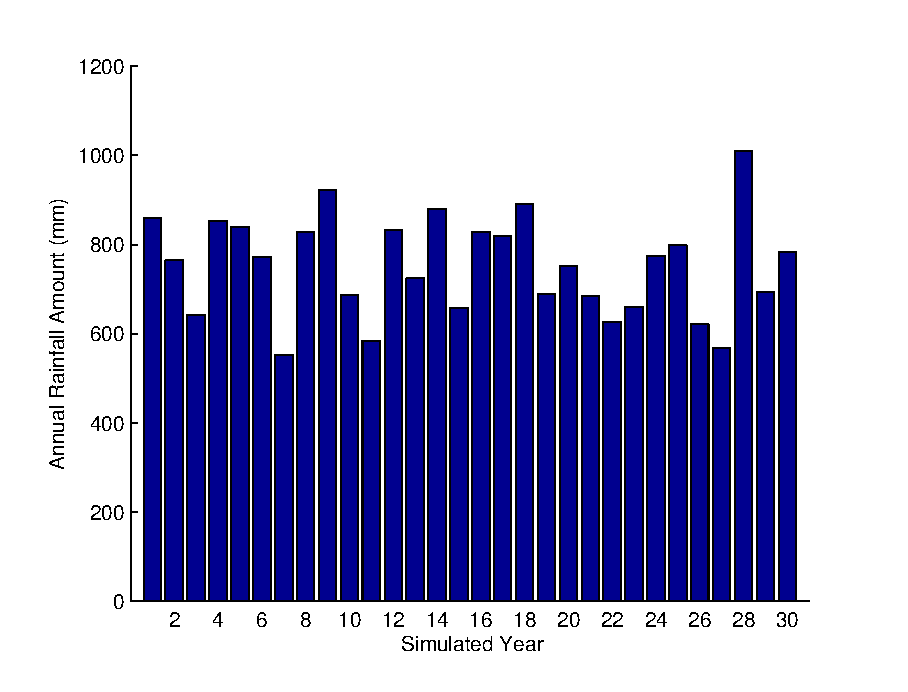
\includegraphics[width=0.60\textwidth]
{./img/annual_future_rainfall}
  \caption{Simulated annual rainfall amount using CLIGEN}
  \label{fig:annual_future_rainfall}
\end{figure}

The changes in mean maximum 30-min peak intensity shows negative relationships,
as expected, with the rainfall duration changes. Every 1\% decrease/increase in
mean maximum 30-min peak intensity of wet seasons results in a 0.75\%
increase/decrease in annual rainfall duration (Figure
\ref{fig:future_rainfall_duration_change}). For the changes in dry season, the
magnitude of the change was more gradual than that of the wet season (Figure
\ref{fig:future_rainfall_duration_change}). Every 1\% change in the peak
intensity of dry season caused a $-$0.45\% change in annual rainfall duration
\ref{fig:future_rainfall_duration_change}.

\begin{figure}[htbp]
  \centering
    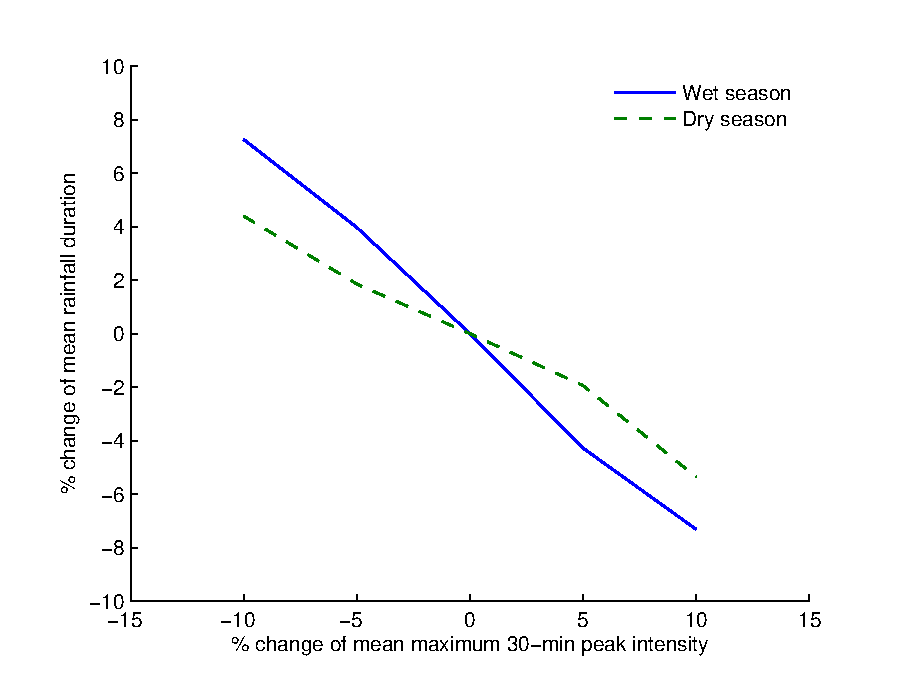
\includegraphics[width=0.60\textwidth]
{./img/future_rainfall_duration_change}
  \caption{Simulated annual rainfall duration changes by changing mean
maximum 30-min peak intensity for wet and dry seasons.}
  \label{fig:future_rainfall_duration_change}
\end{figure}

The changes in average monthly maxima of daily peak intensity for wet and dry
season affected CLIGEN simulated daily peak rainfall intensities (Figure
\ref{fig:future_monthly_intensity}). The changes in average monthly maxima of
daily peak intensity in the wet season resulted in increased or decreased daily
peak intensities for wet months (SONDJF). This was also the case for the dry
months (MAMJJA).

\begin{figure}[htbp]
  \centering
    \subfloat[Wet months (9, 10, 11, 12, 1, 2) with modified
intensity]{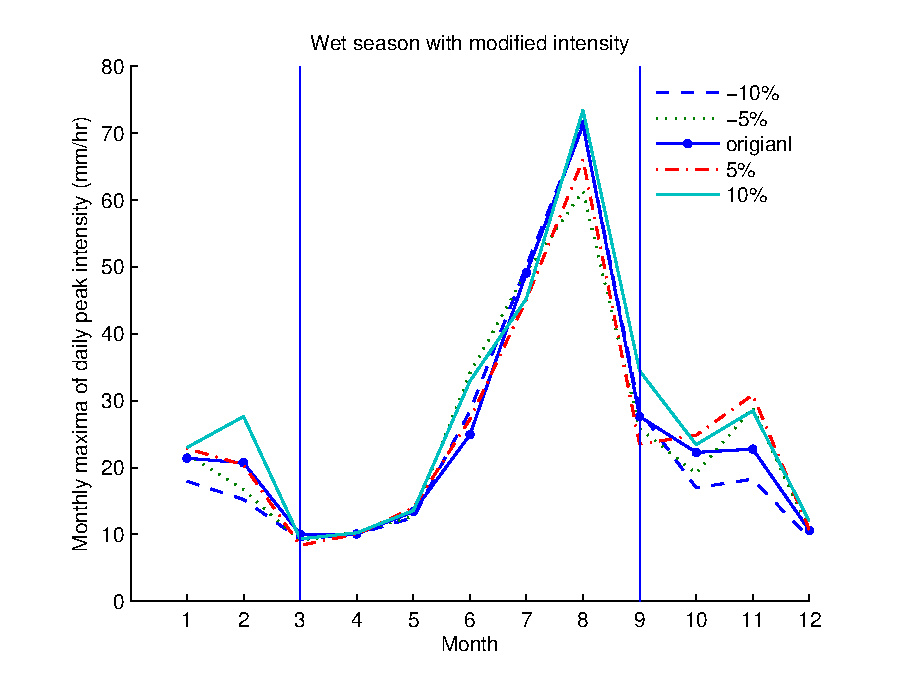
\includegraphics[width=0.70\textwidth]{%
./img/future_monthly_intensity_wet} \label{fig:future_monthly_intensity_wet}}\\
    \subfloat[Dry months (3, 4, 5, 6, 7, 8) with modified
intensity]{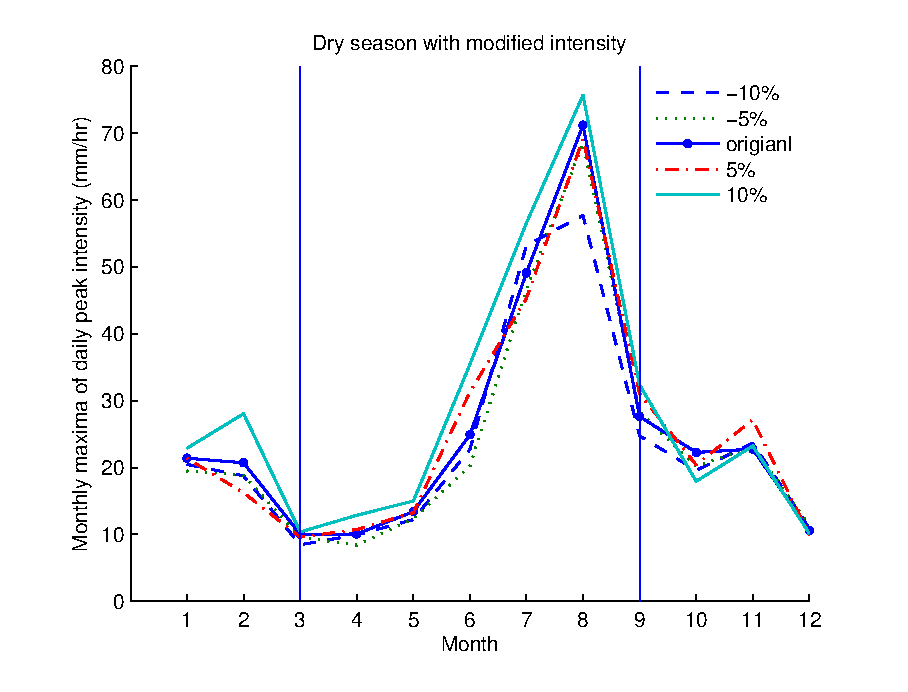
\includegraphics[width=0.70\textwidth]{%
./img/future_monthly_intensity_dry} \label{fig:future_monthly_intensity_dry}}
  \caption{Monthly maxima of daily peak rainfall intensity changes
generated by CLIGEN with modified mean maximum 30-min peak intensity}
  \label{fig:future_monthly_intensity}
\end{figure}

\subsection{Estimated Changes of Future Soil Erosion}
\label{sec:EstimatedFutureSoilErosion}
For the wet season, increases or decreases in mean maximum 30-min peak intensity
generally yield increases or decreases in runoff. Every 1\% change in the mean
maximum 30-min peak intensity for the wet months (SONDJF) resulted in about a
0.72\% change in the mean annual runoff (Figure \ref{fig:future_roff_change}).
For the dry season, 5\% change in mean maximum 30-min peak intensity yield the
greatest changes in runoff (Figure \ref{fig:future_roff_change}) compared to
10\% changes in the intensity. When mean maximum 30-min peak intensity increases
ten per cent, runoff increases, but increases less than that of 5\% change in
the intensity. The similar effect is observed for 10\% decrease in the
intensity.

\begin{figure}[htbp]
  \centering
    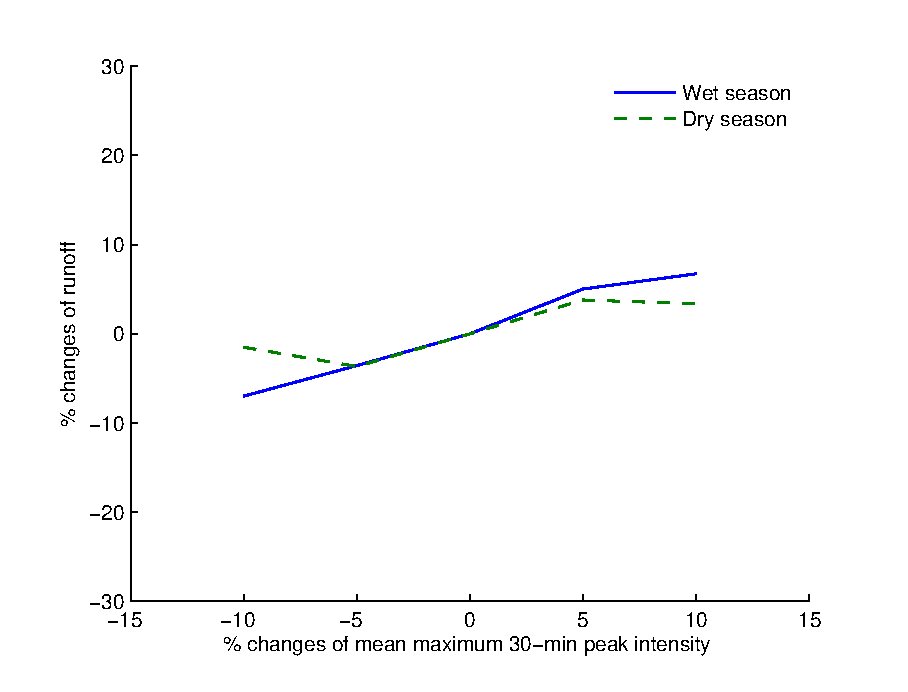
\includegraphics[width=0.6\textwidth]{./img/future_roff_change}
  \caption{Runoff changes in response to the changes of mean maximum
30-min peak intensity for wet and dry seasons.}
  \label{fig:future_roff_change}
\end{figure}

The effect of mean maximum 30-min peak intensity changes on soil loss changes
are more distinctive than on runoff. The effect of the intensity changes in the
wet season and the dry season are markedly different (Figure
\ref{fig:future_sloss_change}). For the wet season, every 1\% increase or
decrease in mean maximum 30-min peak intensity resulted in about a 2\% increase
or decrease in mean annual soil loss rates (Figure
\ref{fig:future_sloss_change}).

The change in mean maximum 30-min peak intensity for dry months show no
significant effect on soil loss rates except a 5\% increase in the intensity
(Figure \ref{fig:future_sloss_change}). When mean maximum 30-min peak intensity
is 5\% increased, average annual soil loss rate increase about a 13.3\% in the
dry season (Figure \ref{fig:future_sloss_change}). This is a 2.7\% increase in
soil loss rate per every 1\% increase in the intensity. This rate of change is
greater than the magnitude of the effect of the intensity changes in the wet
season (i.e.\ a 2\% change in soil loss per every 1\% change in the intensity).

\begin{figure}
  \centering
  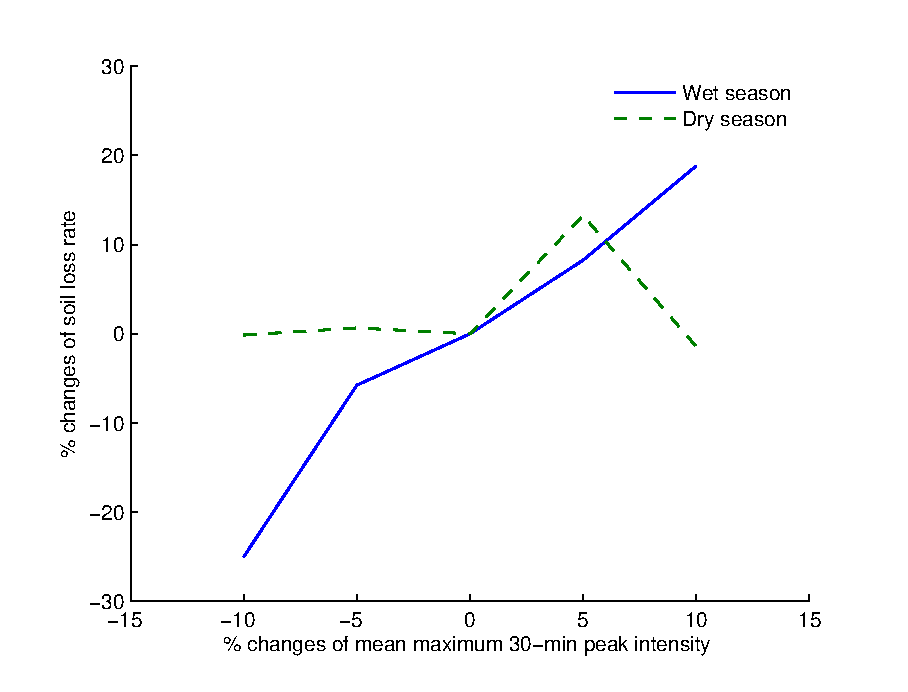
\includegraphics[width=0.6\textwidth]{./img/future_sloss_change}
  \caption{Soil loss rate changes in response to the changes of mean
maximum 30-min peak intensity for wet and dry seasons.}
  \label{fig:future_sloss_change}
\end{figure}

%Individual annual runoff and soil loss rates for the changes of wet and dry
%seasons are presented in Figures \ref{fig:wet_season_roff} to
%\ref{fig:dry_season_sloss}.
%
%\begin{figure}[htbp]
% \centering
%   \subfloat[+10\%]{
%   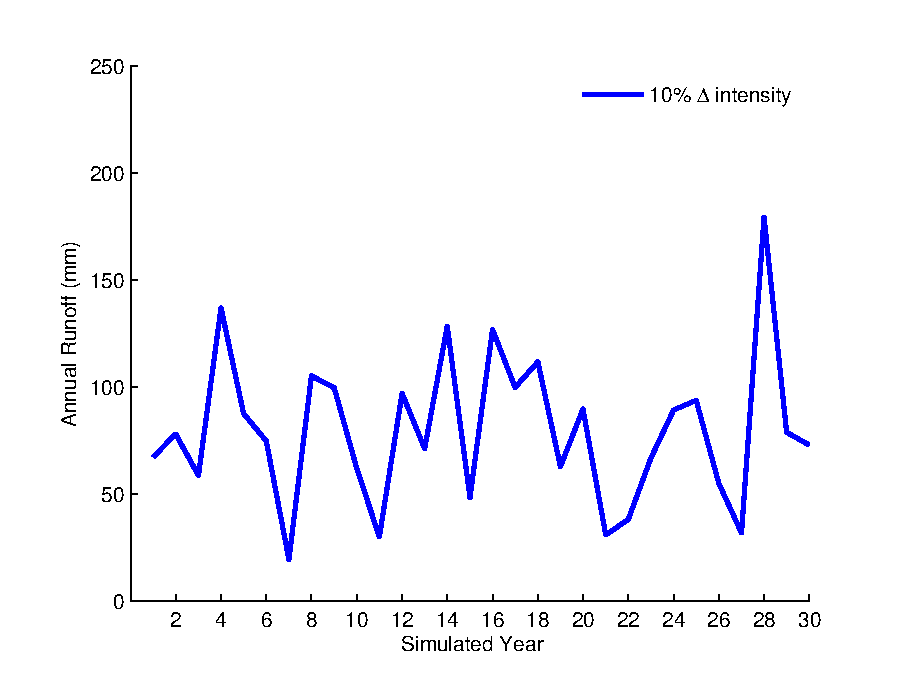
\includegraphics[width=0.45\textwidth]{wet_incr_10_roff}
%   \label{fig:wet_season_roff-a}}
%   \subfloat[+5\%]{
%   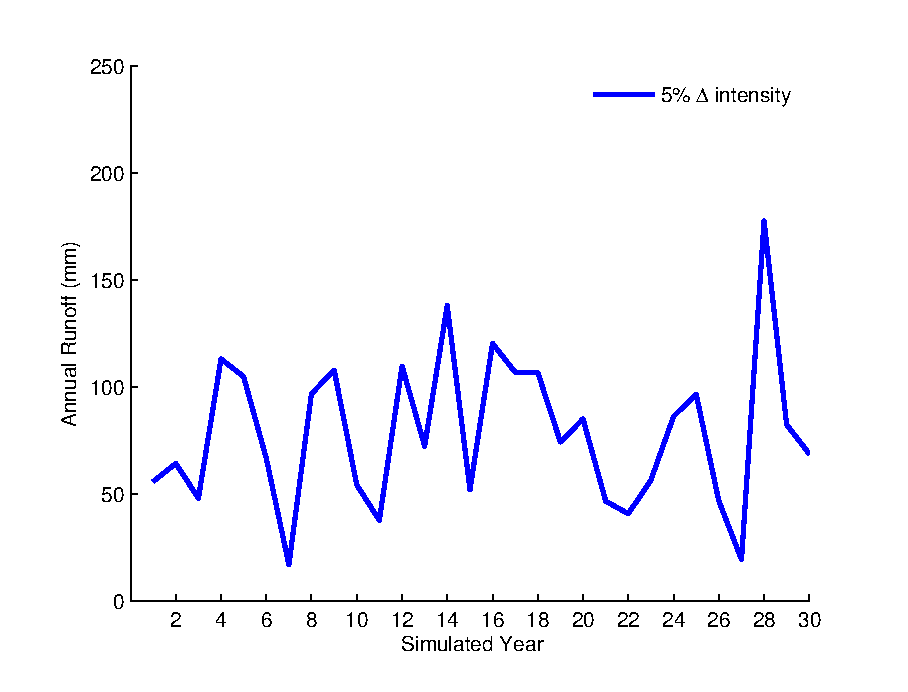
\includegraphics[width=0.45\textwidth]{wet_incr_5_roff}
%   \label{fig:wet_season_roff-b}}
%
%   \subfloat[Original]{
%   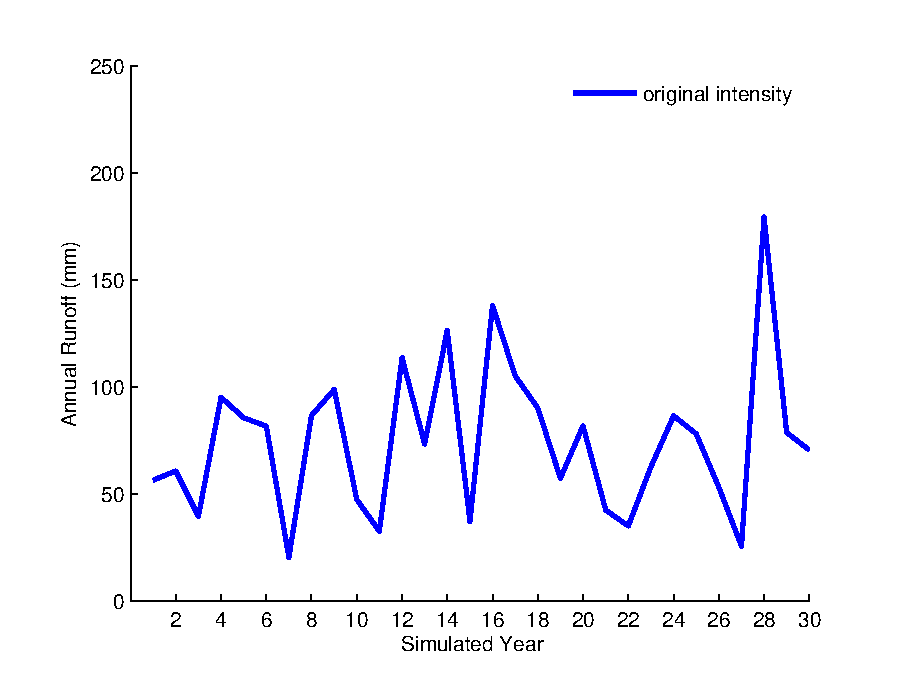
\includegraphics[width=0.45\textwidth]{control_roff}
%   \label{fig:wet_season_roff-c}}
%
%   \subfloat[-5\%]{
%   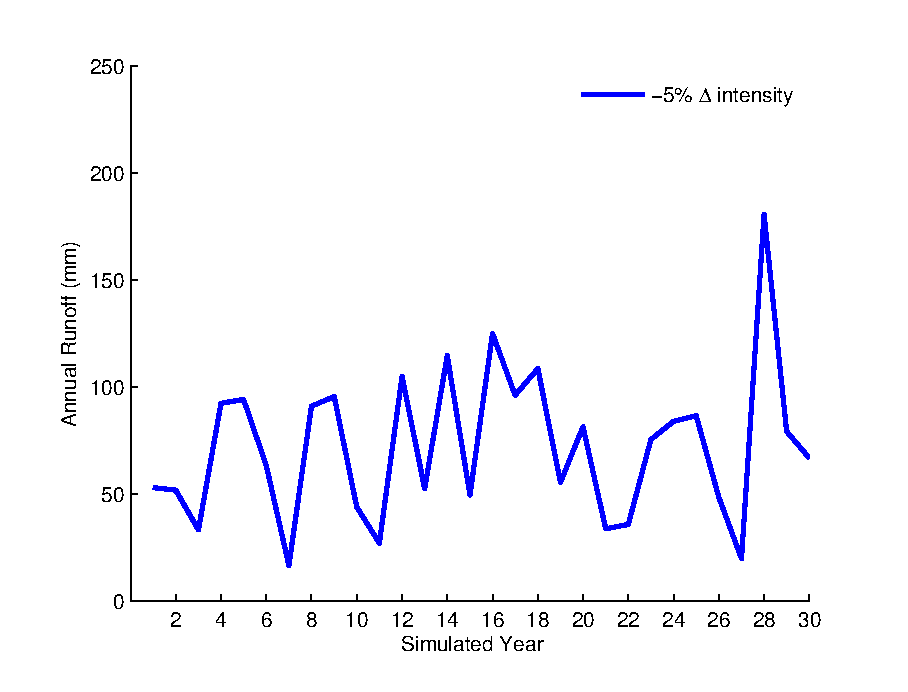
\includegraphics[width=0.45\textwidth]{wet_decr_5_roff}
%   \label{fig:wet_season_roff-d}}
%   \subfloat[-10\%]{
%   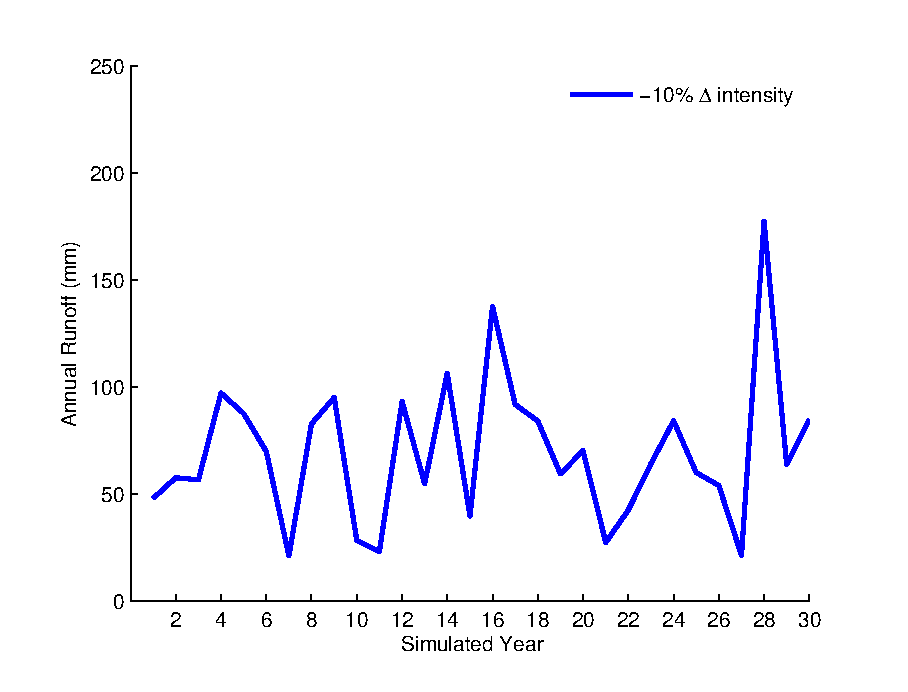
\includegraphics[width=0.45\textwidth]{wet_decr_10_roff}
%   \label{fig:wet_season_roff-e}}
% \caption[Effects of different mean maximum 30-min peak intensity changes
%in wet months on WEPP estimated annual runoff]{Effects of different mean
%maximum 30-min peak intensity changes in wet months (SONDJF) on WEPP
%estimated annual runoff (mm)}
% \label{fig:wet_season_roff}
%\end{figure}
%
%\begin{figure}[htbp]
% \centering
%   \subfloat[+10\%]{
%   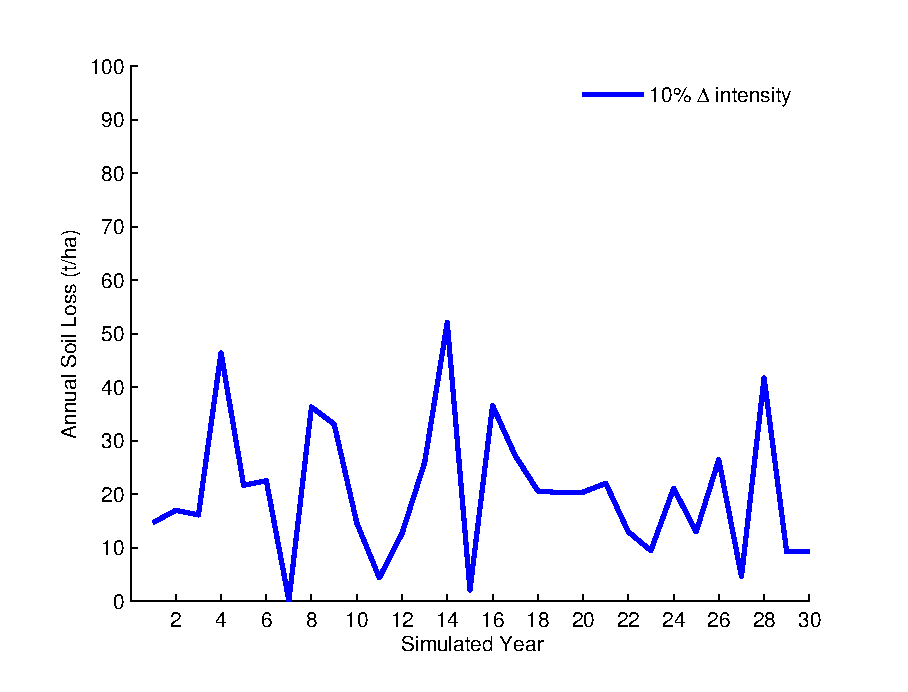
\includegraphics[width=0.45\textwidth]{wet_incr_10_sloss}
%   \label{fig:wet_season_sloss-a}}
%   \subfloat[+5\%]{
%   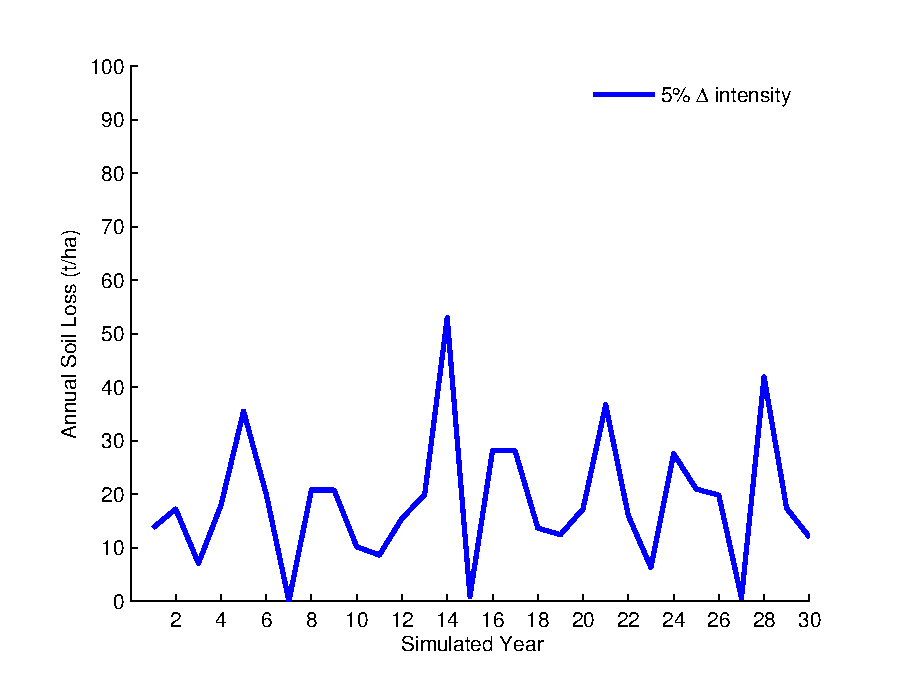
\includegraphics[width=0.45\textwidth]{wet_incr_5_sloss}
%   \label{fig:wet_season_sloss-b}}
%
%   \subfloat[Original]{
%   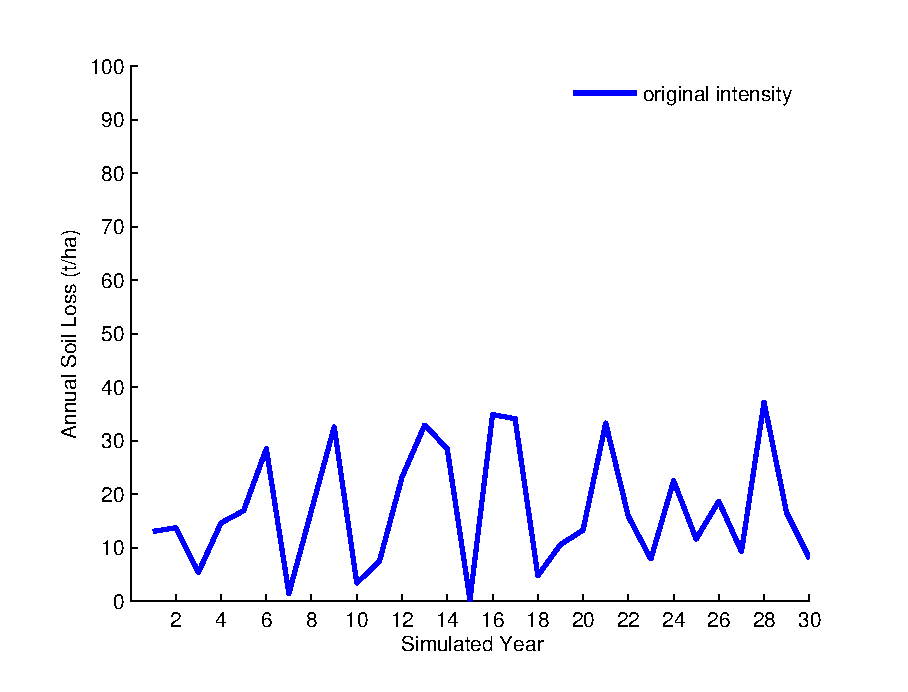
\includegraphics[width=0.45\textwidth]{control_sloss}
%   \label{fig:wet_season_sloss-c}}
%
%   \subfloat[-5\%]{
%   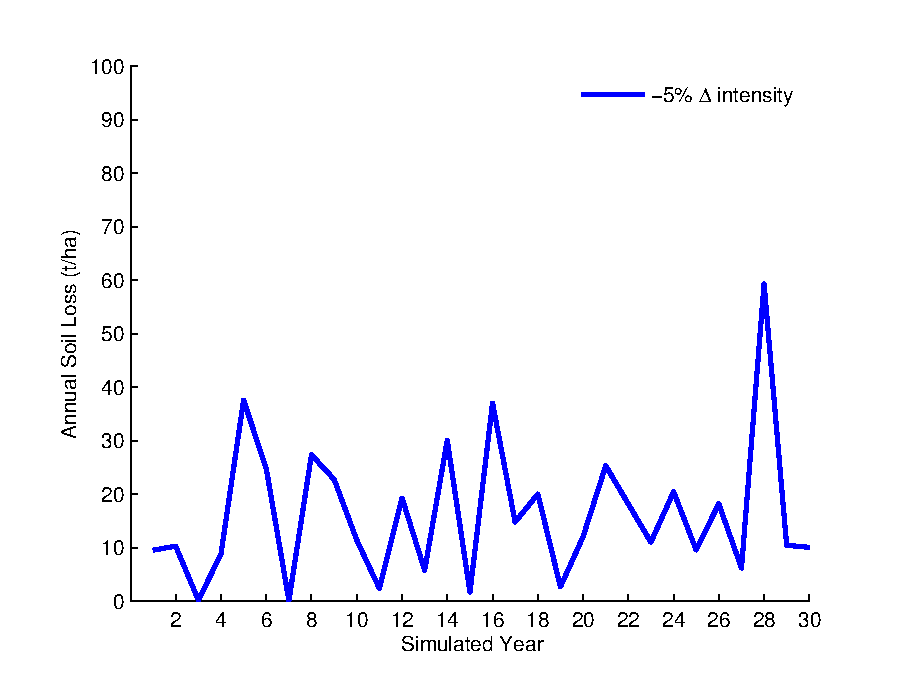
\includegraphics[width=0.45\textwidth]{wet_decr_5_sloss}
%   \label{fig:wet_season_sloss-d}}
%   \subfloat[-10\%]{
%   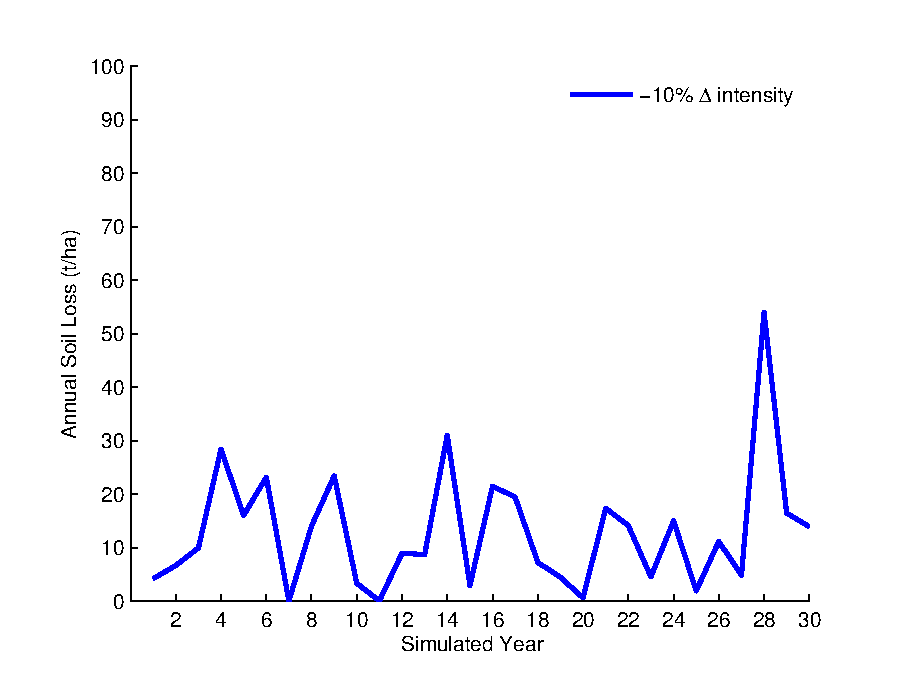
\includegraphics[width=0.45\textwidth]{wet_decr_10_sloss}
%   \label{fig:wet_season_sloss-e}}
% \caption[Effects of different mean maximum 30-min peak intensity changes
%in wet months on WEPP estimated annual soil loss rates]{Effects of
%different mean maximum 30-min peak intensity changes in wet months (SONDJF)
%on WEPP estimated annual soil loss rates (t/ha)}
% \label{fig:wet_season_sloss}
%\end{figure}
%
%\begin{figure}[htbp]
% \centering
%   \subfloat[+10\%]{
%   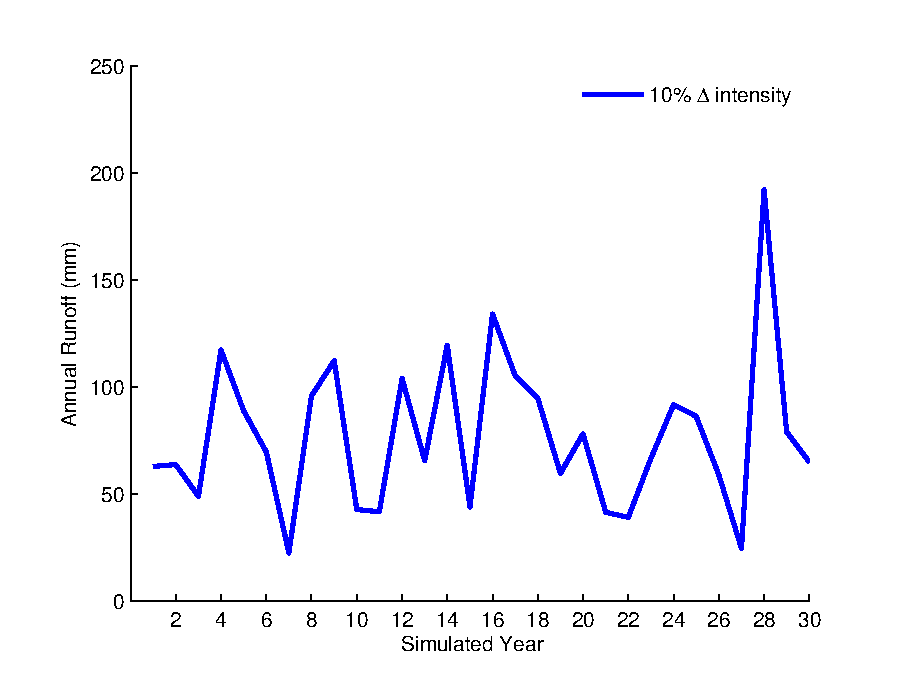
\includegraphics[width=0.45\textwidth]{dry_incr_10_roff}
%   \label{fig:dry_season_roff-a}}
%   \subfloat[+5\%]{
%   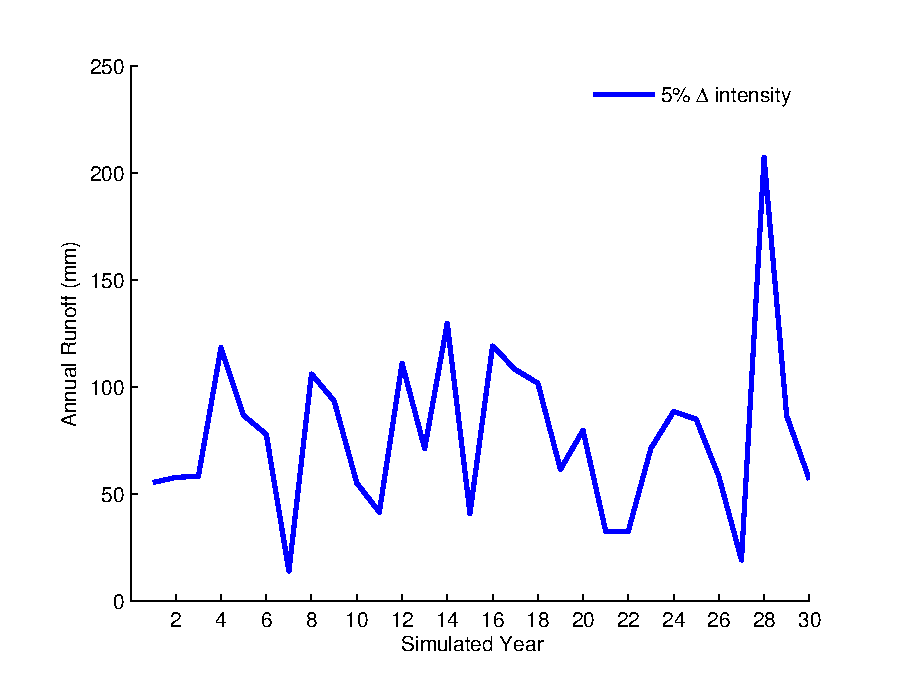
\includegraphics[width=0.45\textwidth]{dry_incr_5_roff}
%   \label{fig:dry_season_roff-b}}
%
%   \subfloat[Original]{
%   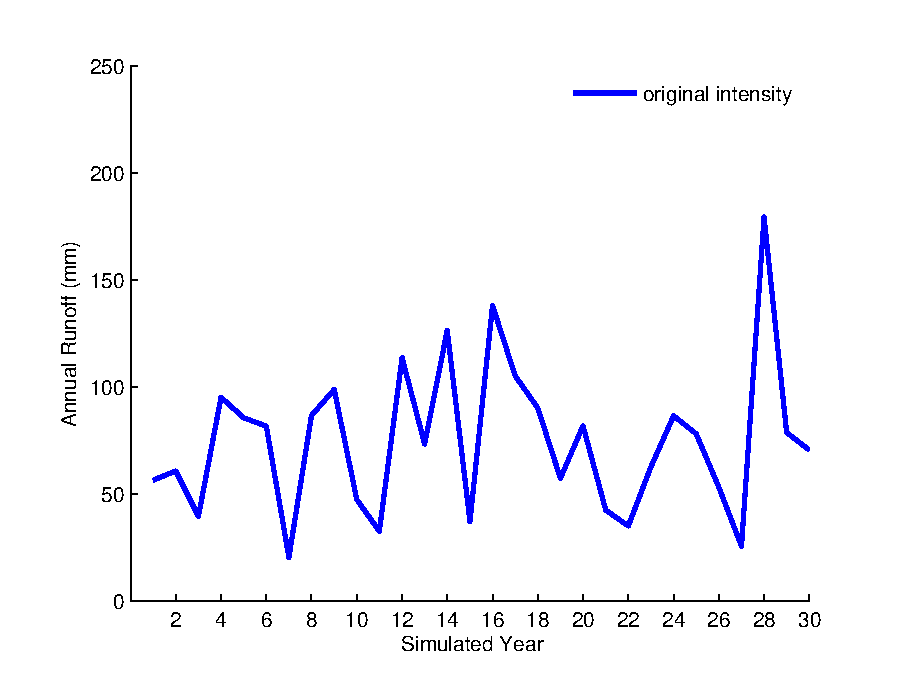
\includegraphics[width=0.45\textwidth]{control_roff}
%   \label{fig:dry_season_roff-c}}
%
%   \subfloat[-5\%]{
%   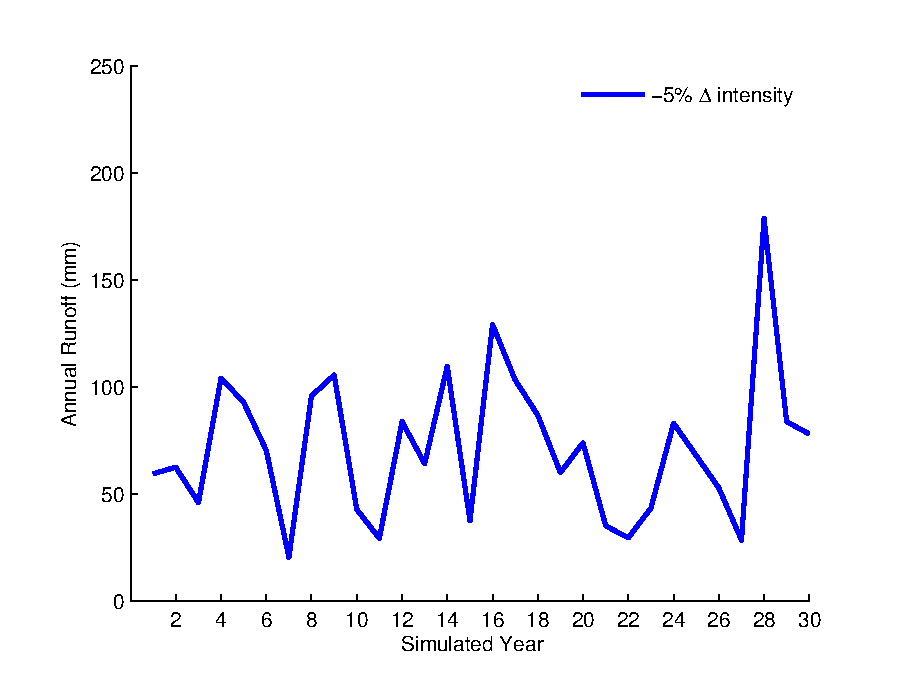
\includegraphics[width=0.45\textwidth]{dry_decr_5_roff}
%   \label{fig:dry_season_roff-d}}
%   \subfloat[-10\%]{
%   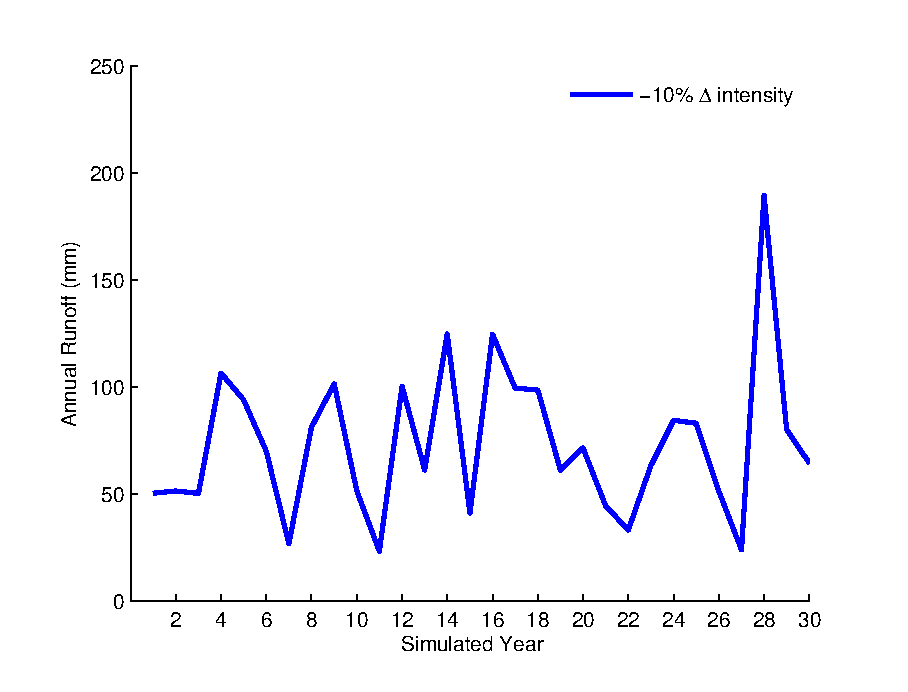
\includegraphics[width=0.45\textwidth]{dry_decr_10_roff}
%   \label{fig:dry_season_roff-e}}
% \caption[Effects of different mean maximum 30-min peak intensity changes
%in dry months on WEPP estimated annual runoff]{Effects of different mean
%maximum 30-min peak intensity changes in dry months (MAMJJA) on WEPP
%estimated annual runoff (mm)}
% \label{fig:dry_season_roff}
%\end{figure}
%
%\begin{figure}[htbp]
% \centering
%   \subfloat[+10\%]{
%   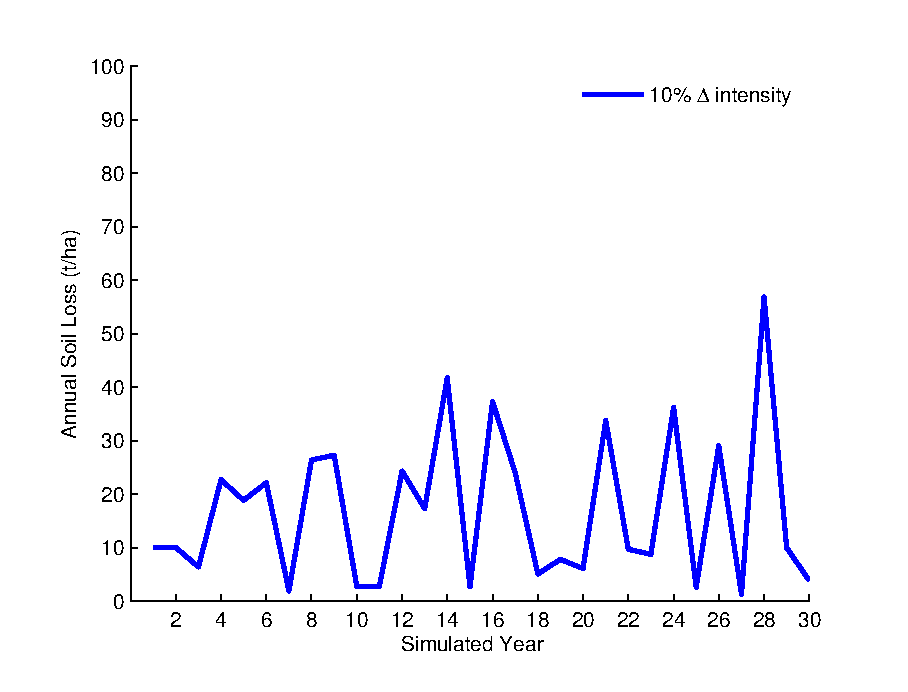
\includegraphics[width=0.45\textwidth]{dry_incr_10_sloss}
%   \label{fig:dry_season_sloss-a}}
%   \subfloat[+5\%]{
%   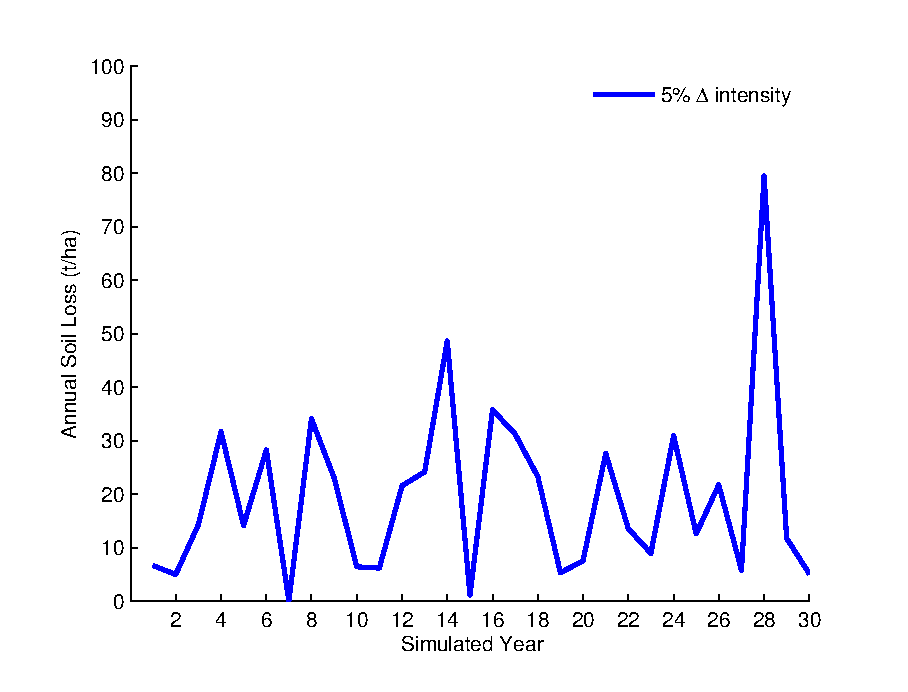
\includegraphics[width=0.45\textwidth]{dry_incr_5_sloss}
%   \label{fig:dry_season_sloss-b}}
%
%   \subfloat[Original]{
%   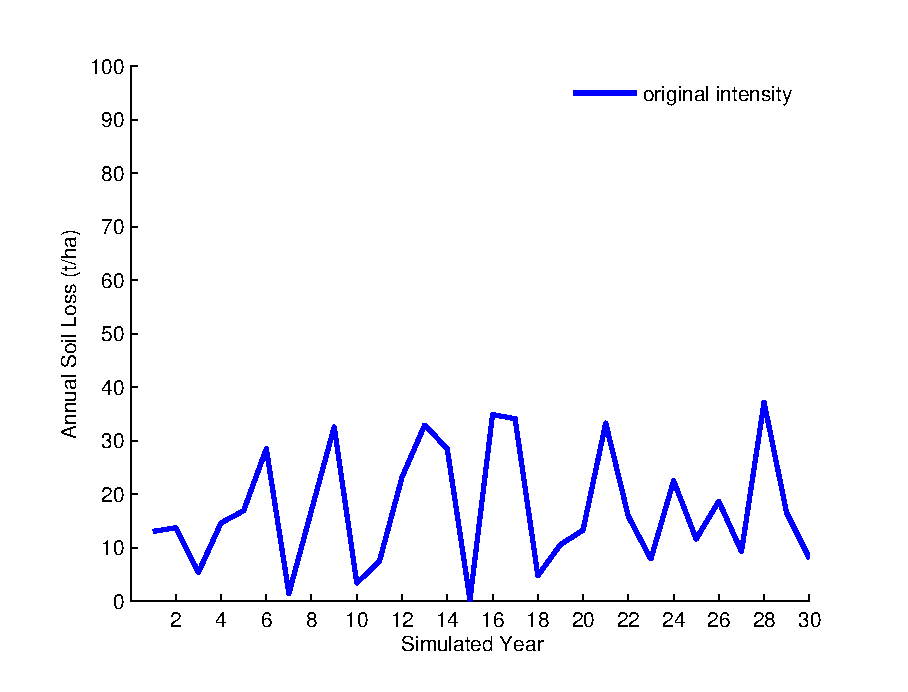
\includegraphics[width=0.45\textwidth]{control_sloss}
%   \label{fig:dry_season_sloss-c}}
%
%   \subfloat[-5\%]{
%   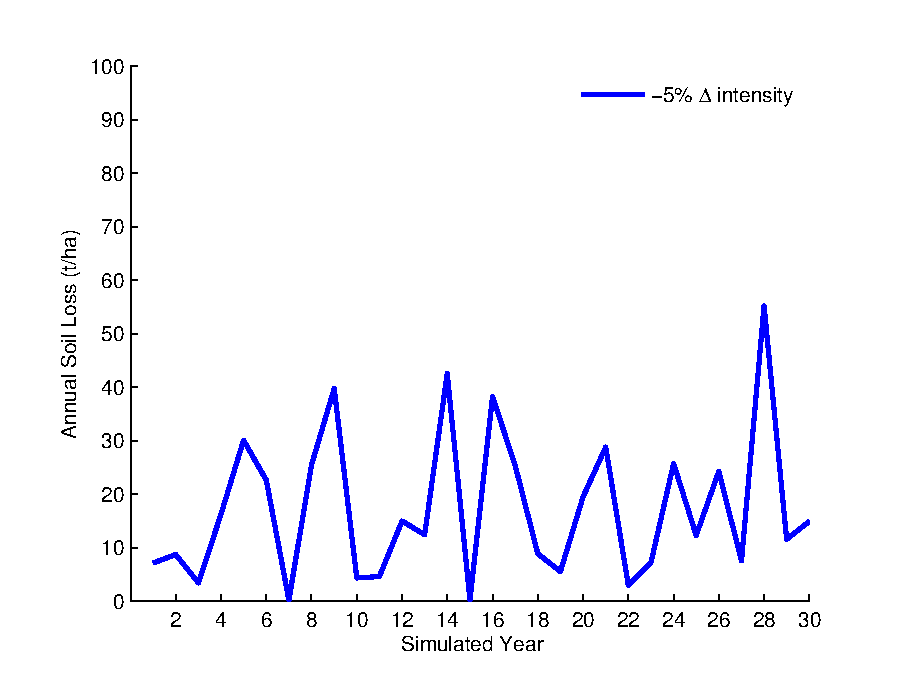
\includegraphics[width=0.45\textwidth]{dry_decr_5_sloss}
%   \label{fig:dry_season_sloss-d}}
%   \subfloat[-10\%]{
%   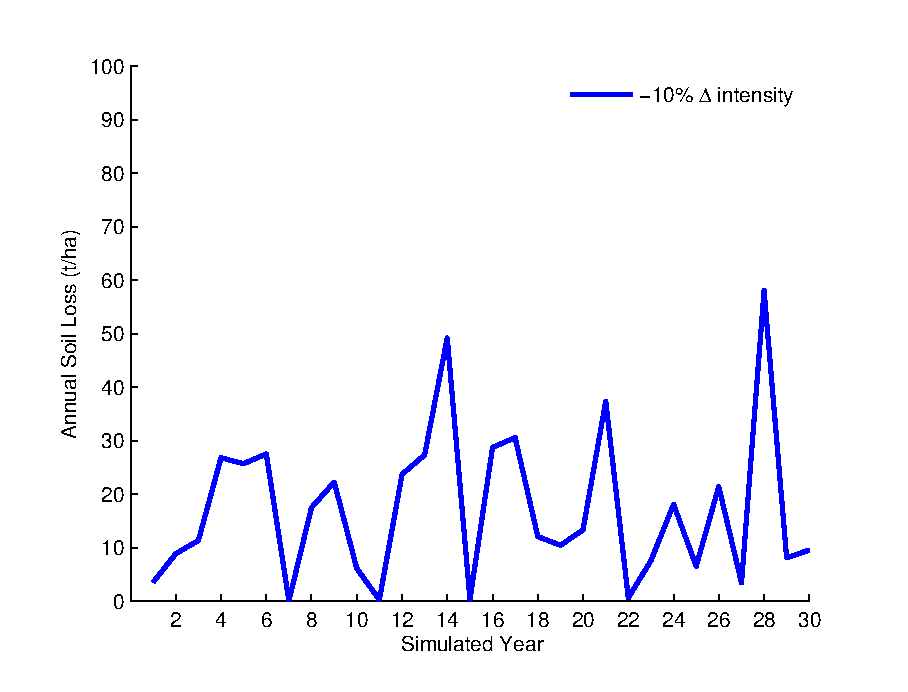
\includegraphics[width=0.45\textwidth]{dry_decr_10_sloss}
%   \label{fig:dry_season_sloss-e}}
% \caption[Effects of different mean maximum 30-min peak intensity changes
%in dry months on WEPP estimated annual soil loss rates]{Effects of
%different mean maximum 30-min peak intensity changes in dry months (MAMJJA)
%on WEPP estimated annual soil loss rates (t/ha)}
% \label{fig:dry_season_sloss}
%\end{figure}


\subsection{Discussion}
\label{sec:EstimationOfFutureSoilErosionDiscussion}

The exceptional response of soil loss rate changes to the 5\% increase in mean
maximum 30-min peak intensity in the dry season are investigated by looking into
event by event simulation results. The 5\% increase in the intensity increases
the number of storm runoff incidents than with original intensity. However,
amount of runoff generated by 5\% increased intensity is slightly (i.e.\ 4\%)
greater than that of the original intensity (mean runoff amount generated per
event is 74.8 mm). This means that each 1\% increase in the intensity resulted
in a 0.8\% increase in runoff. Despite this small differences in runoff amounts,
soil loss rates are 13\% increased in response to 5\% increase in the intensity
in the dry season.

By looking at the number of events which yield soil loss rates more than 15
t/ha, there are 6, 10 and 8 events for the original intensity, 5\% increased
intensity and 10\% increased intensity, respectively (Figure
\ref{fig:event_dry_season_sloss}). There are evidently more incidents of large
erosion events for 5\% increased intensity. However, the differences in number
of erosion event over 15 t/ha are not the result of intensity changes in the dry
season. By looking at the date of each events, far from two events on 29 July in
year 6 and in year 21, all other events occurred in the wet season, mostly in
September, October and November. Also, 29 July is the same date as the harvest
date used for WEPP management input (Table \ref{tab:TillageOperationTiming}).

\begin{figure}[htbp]
  \centering
    \subfloat[Original]{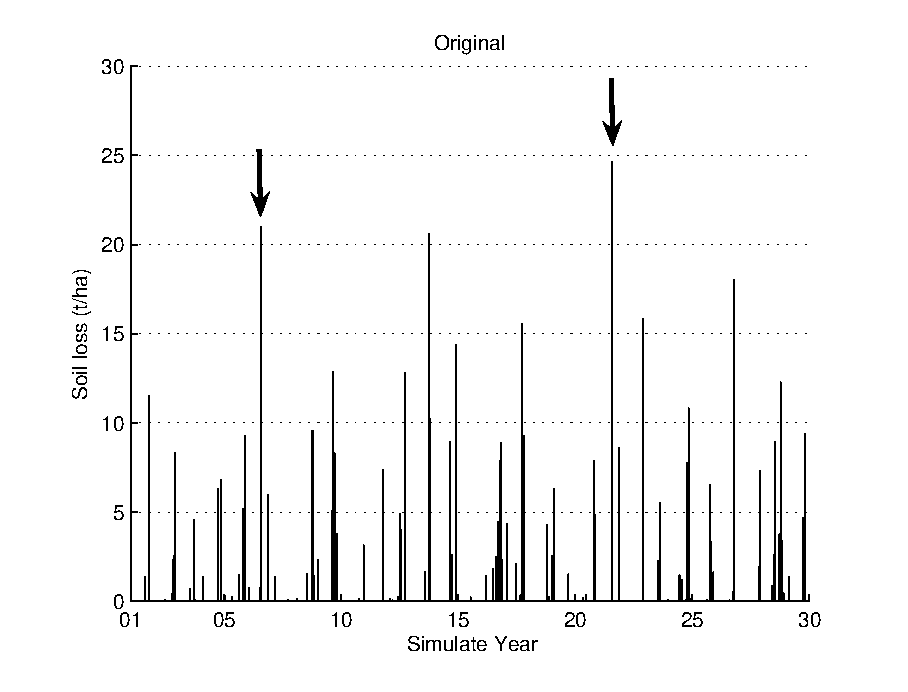
\includegraphics[width=0.5\textwidth]
{./img/event_original} \label{fig:event_dry_season_sloss-c}}\\
    \subfloat[+5\%]{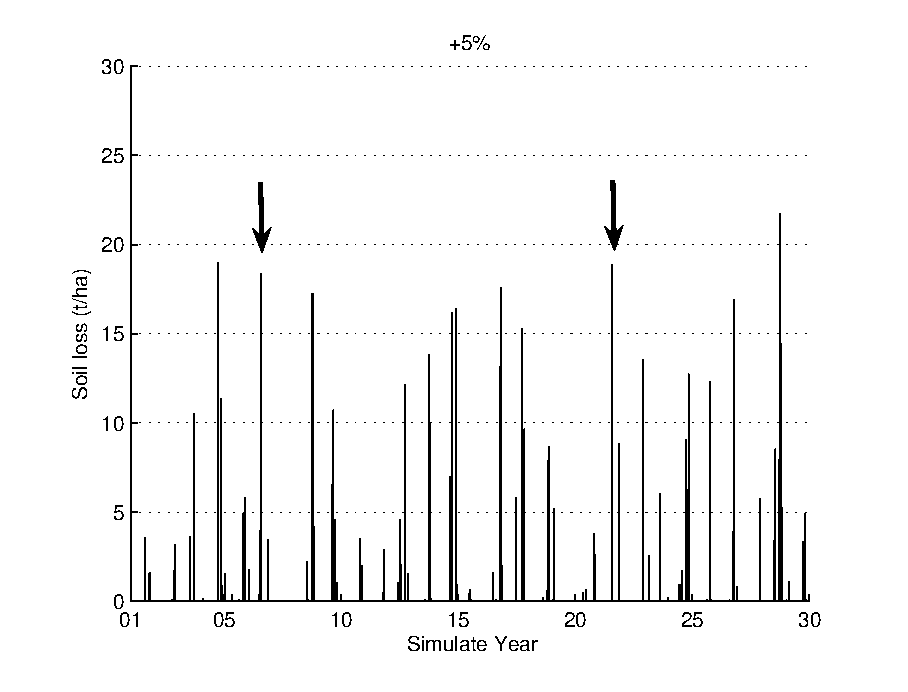
\includegraphics[width=0.5\textwidth]
{./img/event_dry_incr_5} \label{fig:event_dry_season_sloss-b}}\\
    \subfloat[+10\%]{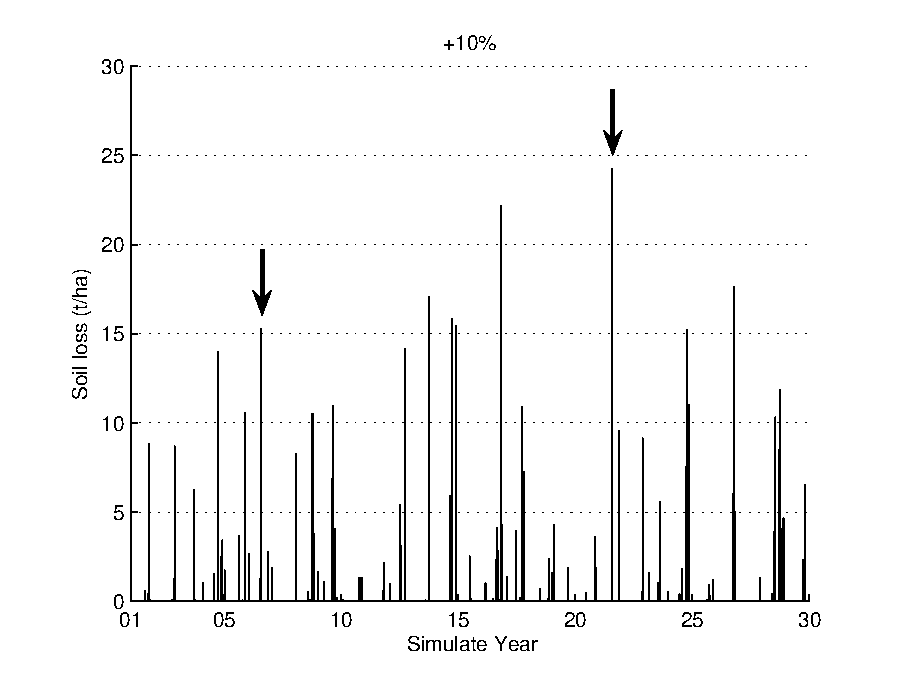
\includegraphics[width=0.5\textwidth]
{./img/event_dry_incr_10} \label{fig:event_dry_season_sloss-a}}
    \caption[Effects of 5\% and 10\% increases of mean maximum
30-min peak intensity on WEPP generated soil loss rates for individual
events]{Effects of 5\% and 10\% increases of mean maximum 30-min peak intensity
on WEPP generated soil loss rates (t/ha) for individual events. The arrows
indicate the erosion events with $>$15 t/ha soil loss on 29 July of year 6 and
year 21.}
  \label{fig:event_dry_season_sloss}
\end{figure}

The intensity increase in dry months is not significantly effective to cause
erosion rate as either they do not have sufficient rainfall amounts to initiate
erosion or surface conditions are not susceptible for erosion because of
sufficient crop covers. The rainfall intensity becomes more important where
other factors such as rainfall amounts are enough to initiate soil erosion.
Thus, intensity increases in the dry months are not effective as intensity
increases in the wet months where rainfall amounts are greater.

The effect of an increase or decrease in monthly mean maximum 30-min peak
intensity in the wet months (SONDJF) are not constrained only to the wet months,
but also slightly to other months---i.e. the dry months (MAMJJA) decreasing or
increasing the peak intensity (Figure \ref{fig:future_monthly_intensity_wet}). A
similar effect is also observed when monthly mean maximum 30-min peak intensity
in the dry months are changed (Figure \ref{fig:future_monthly_intensity_dry}).
This may be due to the fact that CLIGEN attempts to keep the overall rainfall
amount close to the original value.

Each percent change in a peak intensity of extreme events during the wet season
may result in double percent changes in soil loss rates. This is partly due to
WEPP estimates a gradual increase in runoff amount while the number of runoff
events is reduced. As a result of an increased peak intensity during the wet
season, less rainfall events were simulated to retain overall rainfall amount
and number of raindays.

The WEPP simulation results in this chapter suggest that every 1\% increase or
decrease in the mean maximum 30-min peak intensity in the wet season (September
to February) resulted in a 0.72\% increase or decrease in mean annual runoff,
and a 2\% increase or decrease in mean annual soil loss rate.

We do not know precisely what the future rainfall intensity would be like. Even
with climate change models, it is difficult to predict all the rainfall
information required by the present-day erosion models. Without knowing these
rainfall intensity, estimation of future erosion can go wrong easily as shown
previously.
However, using perturbed extreme rainfall intensity will provide a clear and
robust comparisons of soil erosion rates under the conditions where the extreme
rainfall intensity is expected to be increased or decreased.

%compare runoff and erosion rates giving highlight, saying like, `when the
%same magnitude of change occurs in either winter or summer' and such.
%highlight it comparing with the changes occur for the all year with same
%increase/decrease magnitude. Think about the \% changes in Table
%\ref{tab:MX5PChanges}.

%No conclusion may need as there will be one ``conclusion'' for the whole
%chapter.

%arrow (rainfall intensity data) and bow (erosion model)

Despite the availability of various methods we take to predict future rainfall
intensity, predicting soil erosion with good confidence level is almost
impossible (may not be viable) at the moment because the uncertainty involved
for the prediction is too great to be meaningful. As shown in this research,
even with slight different rainfall intensity from the true value---which we may
not be able to know truly---will result in completely different soil erosion
results. However, it is true to say that increased rainfall which may mean---not
necessarily always though---increased erosive power of rainfall and this
increase will result in increased erosion rates.

\section{Conclusion}
\label{sec:EstimatedFutureSoilErosionChapterConclusion}
%This is the conclusion for this chapter.
This chapter aimed to find out the impact of rainfall intensity changes on
future soil erosion by looking at the effect of increased and decreased extreme
rainfall intensity. Two seasonal variations were considered---the wet and dry
season.

The method employed in this chapter successfully generated two different climate
datasets with perturbed monthly rainfall intensity without affecting rainfall
amount and frequency of rainfall. It is important to acquire such dataset in
order to investigate effect of rainfall intensity without compound effects from
other rainfall factors such as amount and frequency of rainfall.

The WEPP simulation results in this chapter suggest that, where the mean maximum
30-min peak intensity in the wet months increases, runoff and soil erosion
increase. Particularly the amount of erosion increases at a even greater rate
than the amount of runoff. The ratio of erosion increases to the rainfall
intensity increase is on the order of 2.

All the figures of simulation outputs from this stage should not be accepted as
``true'' values without careful interpretations. They do not have an adequate
certainty to be accepted directly. It should also be noted that high levels of
uncertainty may be present in the result of the simulation.

%Some will decide that the uncertainty is defined well enough to support their
%decision making; others will decide that the uncertainty is too large to
%support decision making.

%\nolinenumbers
